\PassOptionsToPackage{unicode=true}{hyperref} % options for packages loaded elsewhere
\PassOptionsToPackage{hyphens}{url}
%
\documentclass[a4paper,11pt]{memoir}
%\documentclass[]{article}
\usepackage{lmodern}
\usepackage{amssymb,amsmath}
\usepackage{ifxetex,ifluatex}
\usepackage{fixltx2e} % provides \textsubscript
\ifnum 0\ifxetex 1\fi\ifluatex 1\fi=0 % if pdftex
  \usepackage[T1]{fontenc}
  \usepackage[utf8]{inputenc}
  \usepackage{textcomp} % provides euro and other symbols
\else % if luatex or xelatex
  \usepackage{unicode-math}
  \defaultfontfeatures{Ligatures=TeX,Scale=MatchLowercase}
\fi
% use upquote if available, for straight quotes in verbatim environments
\IfFileExists{upquote.sty}{\usepackage{upquote}}{}
% use microtype if available
\IfFileExists{microtype.sty}{%
\usepackage[]{microtype}
\UseMicrotypeSet[protrusion]{basicmath} % disable protrusion for tt fonts
}{}
\IfFileExists{parskip.sty}{%
\usepackage{parskip}
}{% else
\setlength{\parindent}{0pt}
\setlength{\parskip}{6pt plus 2pt minus 1pt}
}
\usepackage{hyperref}
\hypersetup{
            pdftitle={Cartographical maps and networks},
            pdfauthor={Antonio Rivero Ostoic},
            pdfborder={0 0 0},
            breaklinks=true}
\urlstyle{same}  % don't use monospace font for urls
\usepackage[left=2cm,right=2cm,top=2cm,bottom=2cm]{geometry}
\usepackage{color}
\usepackage{fancyvrb}
\newcommand{\VerbBar}{|}
\newcommand{\VERB}{\Verb[commandchars=\\\{\}]}
\DefineVerbatimEnvironment{Highlighting}{Verbatim}{commandchars=\\\{\}}
% Add ',fontsize=\small' for more characters per line
\usepackage{framed}
\definecolor{shadecolor}{RGB}{248,248,248}
\newenvironment{Shaded}{\begin{snugshade}}{\end{snugshade}}
\newcommand{\AlertTok}[1]{\textcolor[rgb]{0.94,0.16,0.16}{#1}}
\newcommand{\AnnotationTok}[1]{\textcolor[rgb]{0.56,0.35,0.01}{\textbf{\textit{#1}}}}
\newcommand{\AttributeTok}[1]{\textcolor[rgb]{0.77,0.63,0.00}{#1}}
\newcommand{\BaseNTok}[1]{\textcolor[rgb]{0.00,0.00,0.81}{#1}}
\newcommand{\BuiltInTok}[1]{#1}
\newcommand{\CharTok}[1]{\textcolor[rgb]{0.31,0.60,0.02}{#1}}
\newcommand{\CommentTok}[1]{\textcolor[rgb]{0.56,0.35,0.01}{\textit{#1}}}
\newcommand{\CommentVarTok}[1]{\textcolor[rgb]{0.56,0.35,0.01}{\textbf{\textit{#1}}}}
\newcommand{\ConstantTok}[1]{\textcolor[rgb]{0.00,0.00,0.00}{#1}}
\newcommand{\ControlFlowTok}[1]{\textcolor[rgb]{0.13,0.29,0.53}{\textbf{#1}}}
\newcommand{\DataTypeTok}[1]{\textcolor[rgb]{0.13,0.29,0.53}{#1}}
\newcommand{\DecValTok}[1]{\textcolor[rgb]{0.00,0.00,0.81}{#1}}
\newcommand{\DocumentationTok}[1]{\textcolor[rgb]{0.56,0.35,0.01}{\textbf{\textit{#1}}}}
\newcommand{\ErrorTok}[1]{\textcolor[rgb]{0.64,0.00,0.00}{\textbf{#1}}}
\newcommand{\ExtensionTok}[1]{#1}
\newcommand{\FloatTok}[1]{\textcolor[rgb]{0.00,0.00,0.81}{#1}}
\newcommand{\FunctionTok}[1]{\textcolor[rgb]{0.00,0.00,0.00}{#1}}
\newcommand{\ImportTok}[1]{#1}
\newcommand{\InformationTok}[1]{\textcolor[rgb]{0.56,0.35,0.01}{\textbf{\textit{#1}}}}
\newcommand{\KeywordTok}[1]{\textcolor[rgb]{0.13,0.29,0.53}{\textbf{#1}}}
\newcommand{\NormalTok}[1]{#1}
\newcommand{\OperatorTok}[1]{\textcolor[rgb]{0.81,0.36,0.00}{\textbf{#1}}}
\newcommand{\OtherTok}[1]{\textcolor[rgb]{0.56,0.35,0.01}{#1}}
\newcommand{\PreprocessorTok}[1]{\textcolor[rgb]{0.56,0.35,0.01}{\textit{#1}}}
\newcommand{\RegionMarkerTok}[1]{#1}
\newcommand{\SpecialCharTok}[1]{\textcolor[rgb]{0.00,0.00,0.00}{#1}}
\newcommand{\SpecialStringTok}[1]{\textcolor[rgb]{0.31,0.60,0.02}{#1}}
\newcommand{\StringTok}[1]{\textcolor[rgb]{0.31,0.60,0.02}{#1}}
\newcommand{\VariableTok}[1]{\textcolor[rgb]{0.00,0.00,0.00}{#1}}
\newcommand{\VerbatimStringTok}[1]{\textcolor[rgb]{0.31,0.60,0.02}{#1}}
\newcommand{\WarningTok}[1]{\textcolor[rgb]{0.56,0.35,0.01}{\textbf{\textit{#1}}}}
\usepackage{graphicx,grffile}
\makeatletter
\def\maxwidth{\ifdim\Gin@nat@width>\linewidth\linewidth\else\Gin@nat@width\fi}
\def\maxheight{\ifdim\Gin@nat@height>\textheight\textheight\else\Gin@nat@height\fi}
\makeatother
% Scale images if necessary, so that they will not overflow the page
% margins by default, and it is still possible to overwrite the defaults
% using explicit options in \includegraphics[width, height, ...]{}
\setkeys{Gin}{width=\maxwidth,height=\maxheight,keepaspectratio}
\setlength{\emergencystretch}{3em}  % prevent overfull lines
\providecommand{\tightlist}{%
  \setlength{\itemsep}{0pt}\setlength{\parskip}{0pt}}
\setcounter{secnumdepth}{0}
% Redefines (sub)paragraphs to behave more like sections
\ifx\paragraph\undefined\else
\let\oldparagraph\paragraph
\renewcommand{\paragraph}[1]{\oldparagraph{#1}\mbox{}}
\fi
\ifx\subparagraph\undefined\else
\let\oldsubparagraph\subparagraph
\renewcommand{\subparagraph}[1]{\oldsubparagraph{#1}\mbox{}}
\fi

% set default figure placement to htbp
\makeatletter
\def\fps@figure{htbp}
\makeatother

\usepackage{hyperref}
\PassOptionsToPackage{bookmarks=false}{hyperref}

\makeatletter 
\renewcommand{\figurename}{Fig.}
\renewcommand{\thefigure}{\@arabic\c@figure}
\makeatother


\setcounter{page}{25}
\setcounter{figure}{4}

\title{Cartographical maps and networks}
\author{Antonio Rivero Ostoic}
\date{September 2022}

\begin{document}
\maketitle


\begin{Shaded}
\begin{Highlighting}[]
\CommentTok{# load and check versions}
\KeywordTok{library}\NormalTok{(sdam)}
\KeywordTok{packageVersion}\NormalTok{(}\StringTok{"sdam"}\NormalTok{)}
\end{Highlighting}
\end{Shaded}

\begin{verbatim}
[1] '1.0.0'
\end{verbatim}

\hypertarget{cartographical-maps}{%
\section{Cartographical maps}\label{cartographical-maps}}

Cartographical maps of Roman provinces under Emperors Trajan and Hadrian
(year 117AD), and Italian regions under Emperor Augustus (year 27 BC)
are part of the suite of datasets of the \texttt{"sdam"} package. For
instance, four cartographical maps related to the Roman Empire in the
antiquity period are available in dataset \texttt{"retn"} that is loaded
by function \texttt{plot.map()} to depict cartographical maps and
transportation systems. \texttt{plot.map()} is an interface that also
invokes datasets \texttt{"rpmp"} for names and vector shapes of Roman
provinces and regions, and dataset \texttt{"rpmcd"} for including map
captions and dates in the plot.

\hypertarget{political-division}{%
\subsubsection{Political division}\label{political-division}}

Plotting political divisions of the Roman Empire needs the
\texttt{\textquotesingle{}type\textquotesingle{}} argument of function
\texttt{plot.map()} as well.

\begin{Shaded}
\begin{Highlighting}[]
\CommentTok{# Roman provinces}
\KeywordTok{plot.map}\NormalTok{(}\DataTypeTok{type=}\StringTok{"rp"}\NormalTok{)}
\end{Highlighting}
\end{Shaded}

{\centering
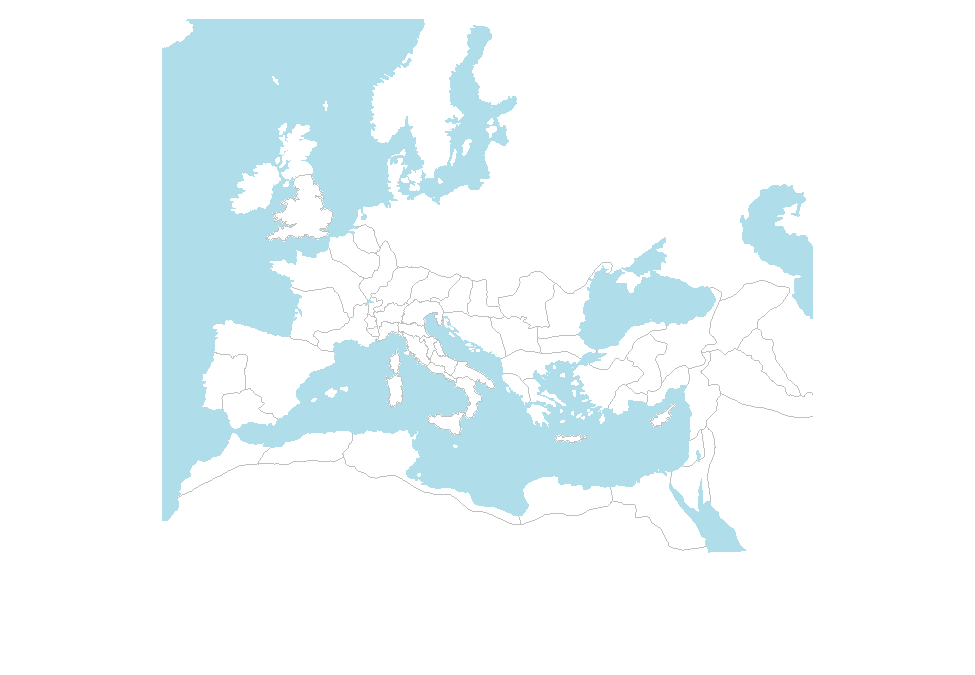
\includegraphics[width=10cm, trim=0 0 0 0, clip]{img/unnamed-chunk-3-1_} 
}

\begin{Shaded}
\begin{Highlighting}[]
\CommentTok{# senatorial/imperial division}
\KeywordTok{plot.map}\NormalTok{(}\DataTypeTok{type=}\StringTok{"si"}\NormalTok{, }\DataTypeTok{main=}\StringTok{"Roman Empire (AD 117)"}\NormalTok{)}
\end{Highlighting}
\end{Shaded}

{\centering
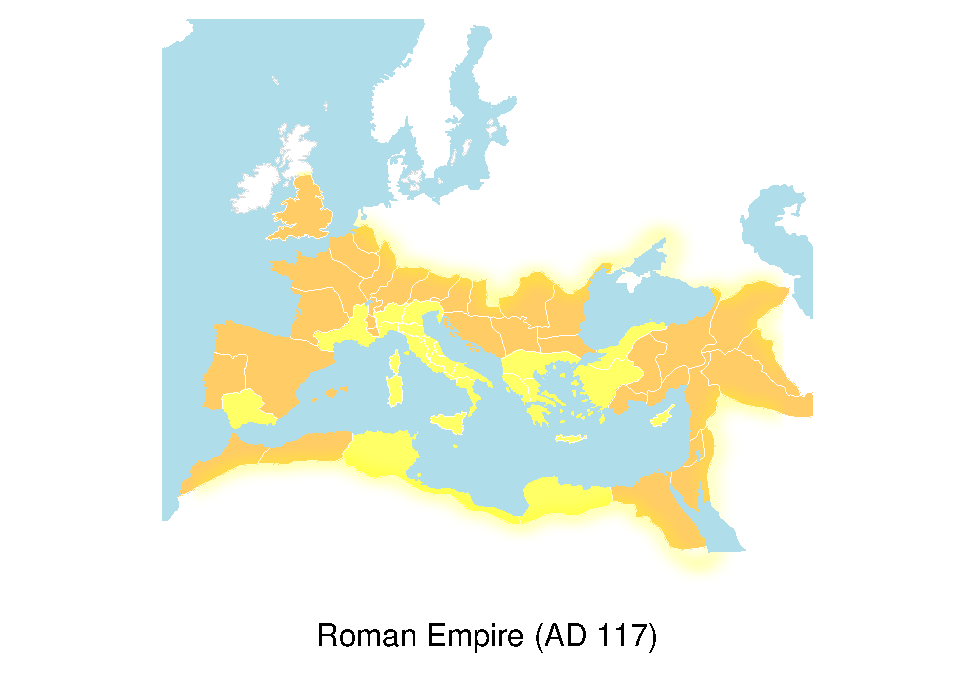
\includegraphics[width=10cm, trim=0 0 0 0, clip]{img/unnamed-chunk-4-1} 
}

\bigbreak
\bigbreak

\hypertarget{roman-provinces-and-regions}{%
\subsubsection{Roman provinces and
regions}\label{roman-provinces-and-regions}}

\begin{itemize}
\tightlist
\item
  Roman provinces and regions shapes and colours for \texttt{plot.map()}
  are in dataset \texttt{"rpmp"}, while the acronyms in \texttt{x} are
  as in dataset \texttt{"rp"}.
\end{itemize}

\begin{Shaded}
\begin{Highlighting}[]
\CommentTok{# Italian peninsula silhouette}
\KeywordTok{plot.map}\NormalTok{(}\DataTypeTok{x=}\StringTok{"Ita"}\NormalTok{)}
\end{Highlighting}
\end{Shaded}

{\centering
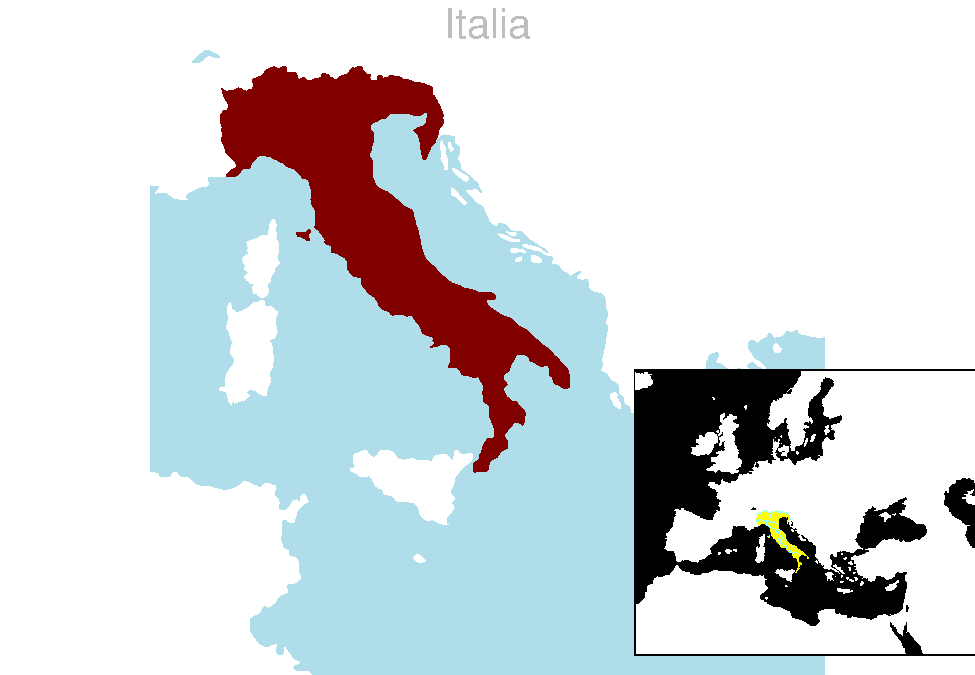
\includegraphics[width=6cm, trim=0 0 0 0, clip]{img/unnamed-chunk-5-1_} 
}

\bigbreak
\bigbreak

\begin{Shaded}
\begin{Highlighting}[]
\CommentTok{# Roman province with establishment date}
\KeywordTok{plot.map}\NormalTok{(}\DataTypeTok{x=}\StringTok{"Bri"}\NormalTok{, }\DataTypeTok{date=}\OtherTok{TRUE}\NormalTok{)}
\end{Highlighting}
\end{Shaded}

{\centering
\includegraphics[width=6cm, trim=0 0 0 0, clip]{img/unnamed-chunk-6-1} 
%\includegraphics{Maps_files/figure-latex/unnamed-chunk-6-1.pdf}
}

\bigbreak
\bigbreak

\begin{Shaded}
\begin{Highlighting}[]
\CommentTok{# Italian region}
\KeywordTok{plot.map}\NormalTok{(}\DataTypeTok{x=}\StringTok{"VeH"}\NormalTok{, }\DataTypeTok{cap=}\OtherTok{FALSE}\NormalTok{, }\DataTypeTok{fsize=}\DecValTok{12}\NormalTok{)}
\end{Highlighting}
\end{Shaded}

{\centering
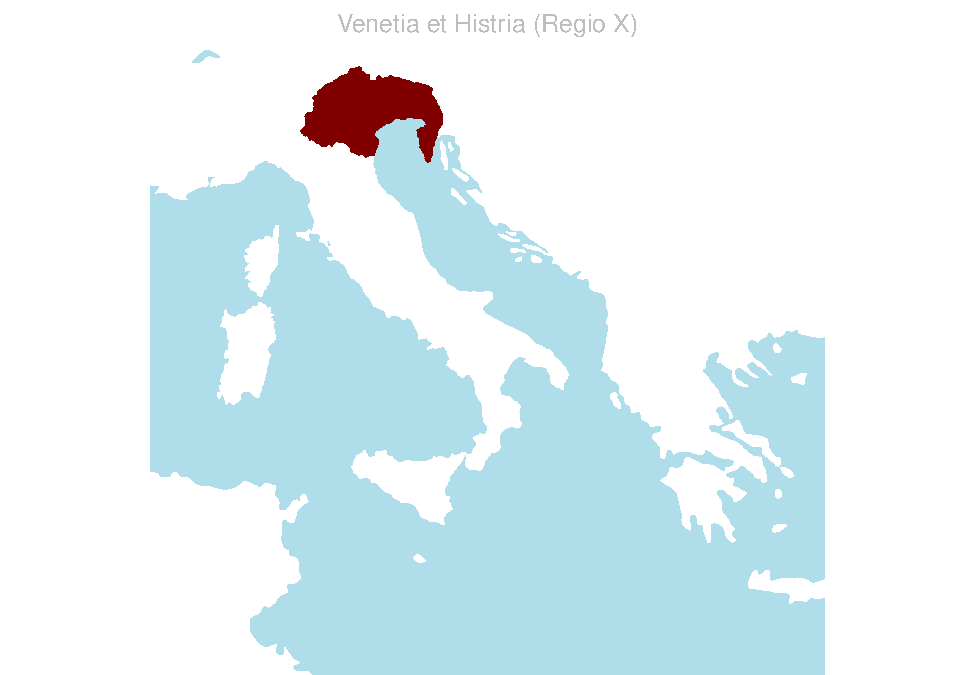
\includegraphics[width=6cm, trim=0 0 0 0, clip]{img/unnamed-chunk-7-1} 
}

\bigbreak
\bigbreak

\hypertarget{transportation-system}{%
\subsection{Transportation system}\label{transportation-system}}

A \texttt{plain} cartographical map with a Roman transportation system
made of settlements and terrestrial and maritime routes is possible with
the \texttt{type} argument in \texttt{plot.map()}, or else by specifying
with arguments \texttt{settl}, \texttt{roads}, and \texttt{shipr} for
the settlements and this routes in the transportation system.

\bigbreak
\bigbreak

\begin{Shaded}
\begin{Highlighting}[]
\CommentTok{# settlements and main roads}
\KeywordTok{plot.map}\NormalTok{(}\DataTypeTok{type=}\StringTok{"plain"}\NormalTok{, }\DataTypeTok{settl=}\OtherTok{TRUE}\NormalTok{, }\DataTypeTok{roads=}\OtherTok{TRUE}\NormalTok{)}
\end{Highlighting}
\end{Shaded}

{\centering
\includegraphics[width=12cm, trim=0 0 0 0, clip]{img/unnamed-chunk-8-1} 
%\includegraphics{Maps_files/figure-latex/unnamed-chunk-8-1.pdf}
}

\begin{Shaded}
\begin{Highlighting}[]
\CommentTok{# settlements and main shipping routes}
\KeywordTok{plot.map}\NormalTok{(}\DataTypeTok{type=}\StringTok{"plain"}\NormalTok{, }\DataTypeTok{settl=}\OtherTok{TRUE}\NormalTok{, }\DataTypeTok{shipr=}\OtherTok{TRUE}\NormalTok{)}
\end{Highlighting}
\end{Shaded}

{\centering
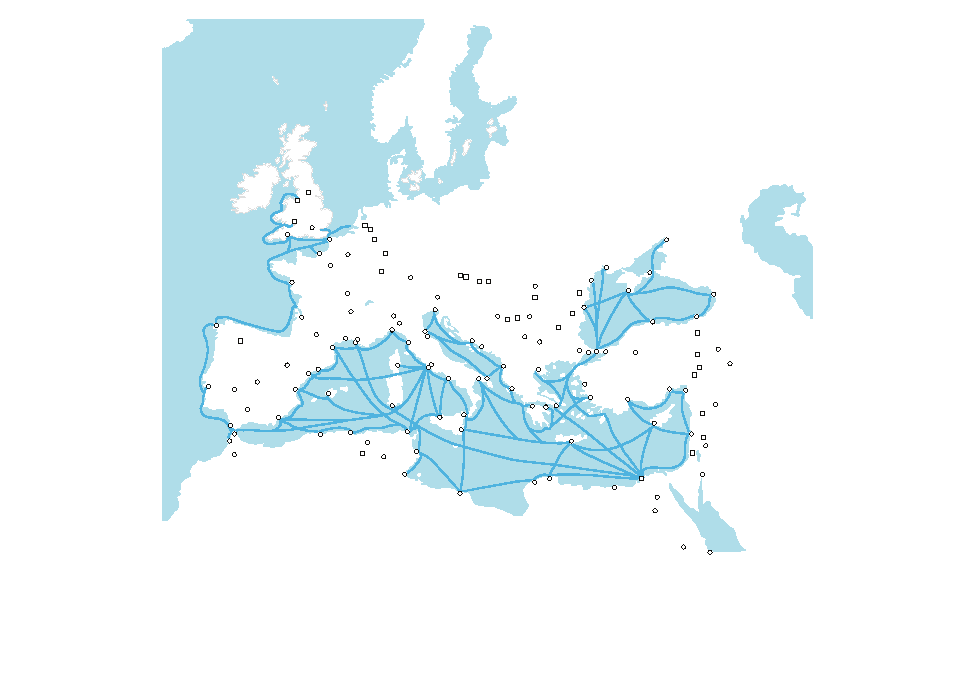
\includegraphics[width=12cm, trim=0 0 0 0, clip]{img/unnamed-chunk-9-1} 
}

\hypertarget{graphs}{%
\section{Graphs}\label{graphs}}

\hypertarget{shipwrecks-network}{%
\subsubsection{Shipwrecks network}\label{shipwrecks-network}}

Graph representations of the transport network is possible with packages
\texttt{"multigraph"} and \texttt{"multiplex"}.

Access to the shipwrecks dataset.

\begin{Shaded}
\begin{Highlighting}[]
\CommentTok{# shipwrecks dataset}
\NormalTok{sw <-}\StringTok{ }\KeywordTok{system.file}\NormalTok{(}\StringTok{"extdata"}\NormalTok{,}\StringTok{"StraussShipwrecks.csv"}\NormalTok{,}\DataTypeTok{package=}\StringTok{"sdam"}\NormalTok{) }\OperatorTok{|}\ErrorTok{>}\StringTok{ }
\StringTok{  }\KeywordTok{read.csv}\NormalTok{(}\DataTypeTok{sep=}\StringTok{";"}\NormalTok{)}
\end{Highlighting}
\end{Shaded}

\begin{Shaded}
\begin{Highlighting}[]
\CommentTok{# variables are checked}
\KeywordTok{colnames}\NormalTok{(sw)}
\end{Highlighting}
\end{Shaded}

\begin{verbatim}
 [1] "Wreck.ID"                "Strauss.ID"              "Name"                   
 [4] "Parker.Number"           "Sea.area"                "Country"                
 [7] "Region"                  "Latitude"                "Longitude"              
[10] "Min.depth"               "Max.depth"               "Depth"                  
[13] "Period"                  "Dating"                  "Earliest.date"          
[16] "Latest.date"             "Date.range"              "Mid.point.of.date.range"
[19] "Probability"             "Place.of.origin"         "Place.of.destination"   
[22] "Reference"               "Comments"                "Amphorae"               
[25] "Marble"                  "Columns.etc"             "Sarcophagi"             
[28] "Blocks"                  "Marble.type"             "Other.cargo"            
[31] "Hull.remains"            "Shipboard.paraphernalia" "Ship.equipment"         
[34] "Estimated.tonnage"       "Amphora.type"           
\end{verbatim}

A system of maritime routes is found in variables
\texttt{Place.of.origin} and \texttt{Place.of.destination}, which
correspond to columns 20 to 21 in \texttt{sw}. This edge list needs some
transformations with functions from packages \texttt{"sdam"} and
\texttt{"multiplex"} to be able to plot the shipwrecks network as a
directed graph with loops with a force directed layout.

\begin{Shaded}
\begin{Highlighting}[]
\CommentTok{# graph of shipwrecks network}
\NormalTok{sw[, }\DecValTok{20}\OperatorTok{:}\DecValTok{21}\NormalTok{] }\OperatorTok{|}\ErrorTok{>}\StringTok{ }
\StringTok{  }\NormalTok{sdam}\OperatorTok{::}\KeywordTok{cln}\NormalTok{(}\DataTypeTok{level=}\DecValTok{2}\NormalTok{, }\DataTypeTok{what=}\KeywordTok{c}\NormalTok{(}\StringTok{"("}\NormalTok{,}\StringTok{")"}\NormalTok{), }\DataTypeTok{case=}\DecValTok{1}\NormalTok{, }\DataTypeTok{na.rm=}\OtherTok{TRUE}\NormalTok{) }\OperatorTok{|}\ErrorTok{>}\StringTok{ }
\StringTok{  }\NormalTok{multiplex}\OperatorTok{::}\KeywordTok{transf}\NormalTok{(}\DataTypeTok{type=}\StringTok{"toarray"}\NormalTok{) }\OperatorTok{|}\ErrorTok{>}\StringTok{ }
\StringTok{  }\NormalTok{multigraph}\OperatorTok{::}\KeywordTok{multigraph}\NormalTok{(}\DataTypeTok{layout=}\StringTok{"force"}\NormalTok{, }\DataTypeTok{seed=}\DecValTok{123}\NormalTok{, }\DataTypeTok{loops=}\OtherTok{TRUE}\NormalTok{, }\DataTypeTok{ecol=}\DecValTok{4}\NormalTok{, }\DataTypeTok{sel=}\StringTok{"Rome"}\NormalTok{)}
\end{Highlighting}
\end{Shaded}

{\centering
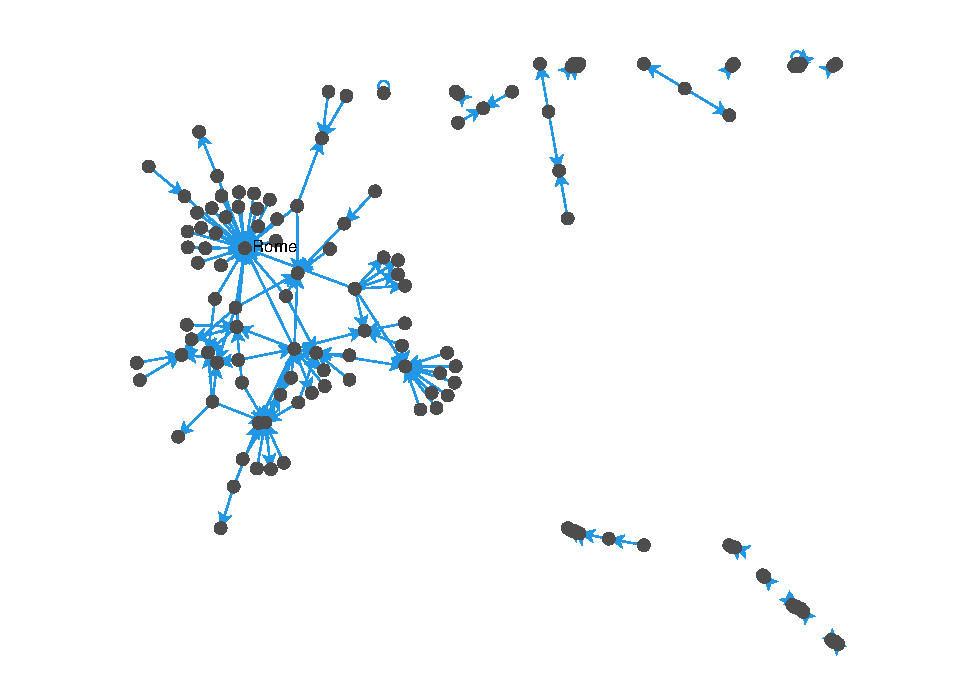
\includegraphics[width=11cm, trim=0 0 0 0, clip]{img/unnamed-chunk-12-1} 
}

In this case, a single node is labeled in the graph that represents the
shipwrecks network without missing information. To keep records with
\texttt{NA} in the data, function \texttt{cln()} has the
\texttt{\textquotesingle{}na.rm\textquotesingle{}} argument to be set to
\texttt{FALSE}.

\bigbreak
\bigbreak

References for shipwrecks data are in

\begin{itemize}
\tightlist
\item
  Vignette: \href{https://cran.r-project.org/web/packages/sdam/vignettes/Intro.html}{Datasets in \texttt{"sdam"} package}
\end{itemize}


\bigbreak
\bigbreak

\hypertarget{see-also}{%
\subsubsection{See also}\label{see-also}}


\begin{itemize}
\tightlist
\item
  \href{https://github.com/mplex/cedhar/blob/master/typesetting/reports/sdam.pdf}{\texttt{"sdam"}
  manual}
\item
  \href{https://CRAN.R-project.org/package=sdam}{\texttt{sdam}: Social Dynamics and
  Complexity in the Ancient Mediterranean}
\end{itemize}

\hypertarget{project}{%
\paragraph{Project}\label{project}}

\begin{itemize}
\tightlist
\item
  \href{https://github.com/sdam-au/sdam}{Release candidate version}
\item
  \href{https://github.com/sdam-au/R_code}{Code snippets using
  \texttt{"sdam"}}
\item
  \href{https://sdam-au.github.io/sdam-au/}{sdam: Digital Tools for the SDAM
  Project at Aarhus University}
\end{itemize}

~

\end{document}
